% !TEX encoding = UTF-8
% !TEX TS-program = pdflatex
% !TEX root = ../Tesi.tex
% !TEX spellcheck = en-EN

%************************************************
\chapter{Motivation and Insufficiency of the State of the Art}
\label{cap:insufficiency}
%************************************************

This work focused on the particles handled by metallurgical industries.
\improvement{list of metallurgical processes with particulate materials. E.g.,
blast furnace is fed with coke and sintered iron ore particles: distribution of
the feed by the chute, raceway formation} 
\improvement{More words on motivation:
industrial processes.
1)Ask MB brochure on sinter cooler. 2) Ask TL and CF material on raceway (cite Alice's thesis).} 

\section{Materials}
\label{sec:materials}

A univocal
method to characterize these particles has so far not been established.
From the experimental point of view, the main issues are the difficult setups and the general 
reliability and reproducibility of the tests. 
From the numerical point of view, no general procedure is available, and the existence of a 
mathematically unique solution describing macro/micro particle contact has yet to be proved.
Moreover, in a recent study, \citet{RefWorks:56} implied "that the dynamic properties of a 
powder cannot be applied to universally predict the static properties of a powder, and, likewise, 
the static properties cannot be used to predict dynamic properties".\\

\section{DEM Simulations}
\label{sec:demsimulations}

In their original formulation of \acs{DEM}, the discrete element method used in
this work, \citet{RefWorks:172} allowed two particles to slightly overlap upon
contact, see Fig. \ref{fig:062collision}, and consequently they proposed
repulsive forces in relation to this overlap distance.
The force that particle $i$ exerts on particle $j$ is defined as:
\begin{equation}
m \ddot{x}_{ij} + c \dot{x}_{ij} + k x_{ij} =  F_{ij} .
\label{equ:newtonlaw}
\end{equation}

\begin{figure}[!htb]
\centering
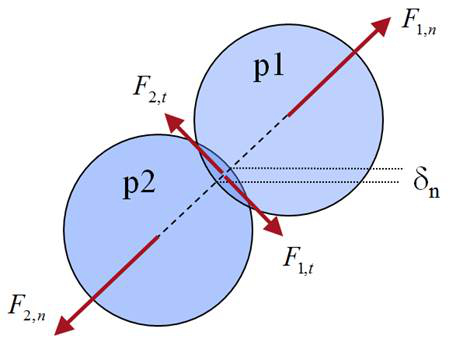
\includegraphics[width=.50\columnwidth]{images/062collision}
\caption[Soft sphere model]{Soft sphere model.}
\label{fig:062collision}
\end{figure}
\improvement{explain why we use DEM}
Their fundamental modelling concept of \acs{DEM} has
since been widely accepted in the literature and their soft sphere contact law has been developed further by
numerous researchers (Vu-Quoc and Zhang \cite{RefWorks:148} and Di Renzo and Di Maio \cite{RefWorks:145}). 
With increasing computational resources, \acs{DEM} simulations have become very
popular giving rise to the development of commercial (e.g., $PFC3D$, used by
Wensrich and Katterfeld \cite{RefWorks:87}) and open-source software (e.g.,
\acs{LIGGGHTS}, Kloss et al. \cite{RefWorks:136}, Aigner et al. \cite{RefWorks:139}).
Soft-sphere \acs{DEM} simulations of thousands of particles have been proven to 
faithfully model particle bulk behaviour, as in Fig. \ref{fig:061cfdemsim}
(Hohner et al. \cite{RefWorks:86}).\\
\begin{figure}[!htb]
\centering
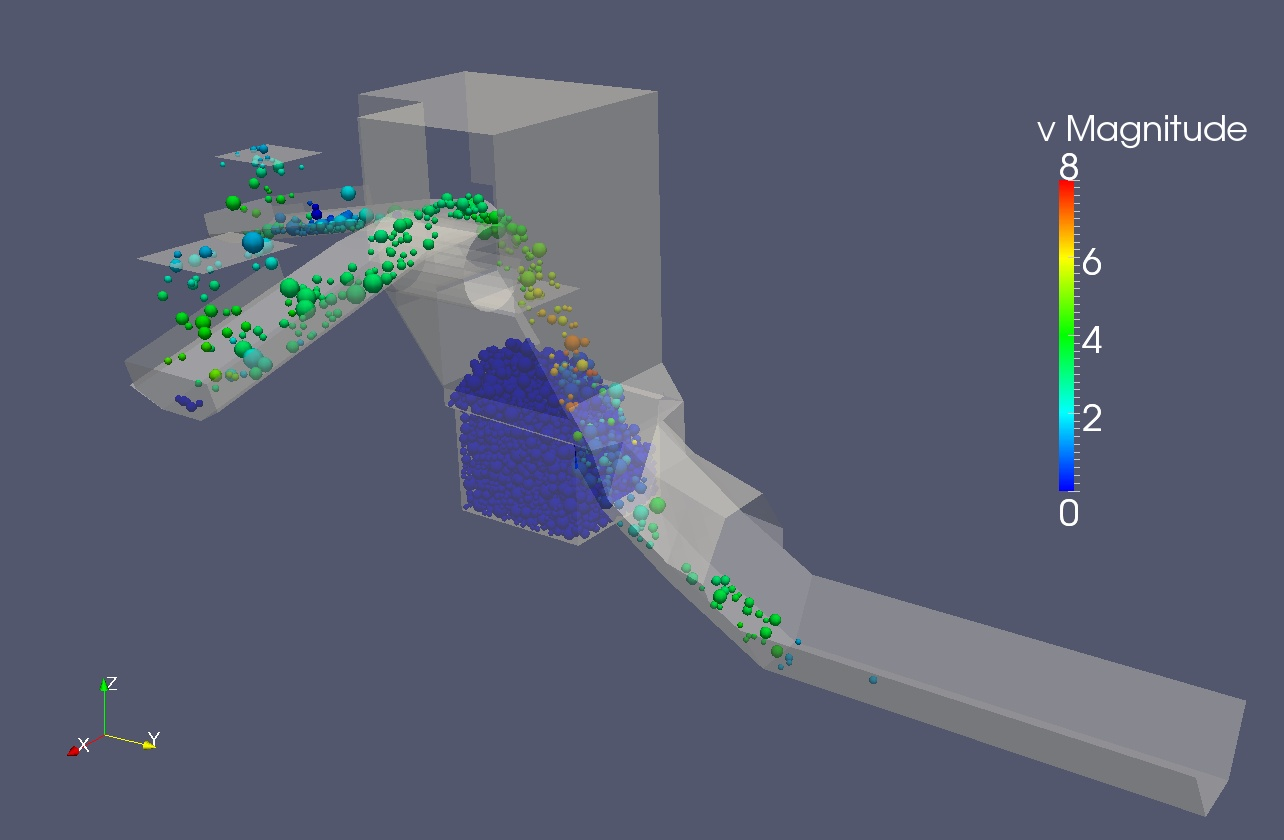
\includegraphics[width=.70\columnwidth]{images/061cfdemsim}
\caption[DEM simulation]{Example of a DEM simulation (www.cfdem.com).}
\label{fig:061cfdemsim}
\end{figure} 

\section{Parameters}
\label{sec:parameters}

In these macroscopic \acs{DEM} simulations, the contact law kernel between a 
pair of particles determines the global bulk behaviour of the granular material (Ai et al. \cite{RefWorks:131}). 
As a consequence, defining a correct contact law is of crucial importance for the predictive 
capability of \acs{DEM} simulations. 
Since \acs{DEM} contact laws are based 
on a set of semi-empirical parameters, correct contact law 
parameters must be defined for a given granular material
or \acs{DEM} simulations will fail (Combarros et al. \cite{RefWorks:177}). \\
Identifying \acs{DEM} contact law parameters is not a trivial task. 
Due to the huge number of particles in a granular material, it
may be impractical to identify valid parameter sets by performing bilateral 
particle collision experiments. 
Furthermore, some contact law parameters such as the coefficient of rolling
friction are purely empirical and cannot be determined by direct 
particle-to-particle measurements (Wensrich and Katterfeld \cite{RefWorks:87}).
Therefore, \acs{DEM} contact law parameters (Table \ref{tab:08DEMparameters}) are
commonly determined by comparing the macroscopic outcome of large-scale \acs{DEM}
simulations with bulk experiments (Alenzi et al. \cite{RefWorks:91}). 
If \acs{DEM} simulation results disagree with bulk measurements, the set of contact
law parameters must be adjusted until reasonable agreement is achieved.\\
However, this purely forward methodology of parameter identification is limited by 
the multi-dimensionality of the parameter space and the associated computational costs of the required 
\acs{DEM} test simulations. 
Moreover, one parameter set which is valid for one bulk behaviour (e.g., angle
of repose) might fail for another (e.g., shear tester). \\
There are yet ways to determine contact parameters directly by measuring
material properties or by performing particle based experiments, see e.g. Combarros et al. \cite{RefWorks:177}, 
Paulick et al. \cite{RefWorks:181}, and Lommen et al. \cite{RefWorks:186}. 
However, these methodologies are laborious, 
since they have to be performed for every new granular material prior to a \acs{DEM}
simulations. 
Especially for the already cited rolling friction parameter, it is arduous to
link the rolling friction parameter to the non-sphericity of the particle. Clearly, there is a
need for an efficient method for identifying \acs{DEM} contact law parameters, given
a specific particle behaviour.



